\chapter{Конструкторская часть}

\section{Схема алгоритма нахождения расстояния Левенштейна}
На рисунке \ref{scheme:levrec} приведена схема рекурсивного алгоритма нахождения
расстояния Левенштейна.
На рисунках \ref{scheme:levrecmemoutter} - \ref{scheme:levrecmeminner} приведены схемы рекурсивного алгоритма нахождения расстояния Левенштейна с кэшированием.


\section{Схема алгоритма нахождения расстояния Дамерау-Левенштейна}
На рисунках \ref{scheme:damlevrectop} - \ref{scheme:damlevrecbottom} приведена схема рекурсивного алгоритма нахождения расстояния Дамерау-Левенштейна.
На рисунках \ref{scheme:damlevmatrtop} - \ref{scheme:damlevmatrbottom} приведена схема итерационного алгоритма нахождения расстояния Дамерау-Левенштейна.


\begin{figure}[h]
	\centering
	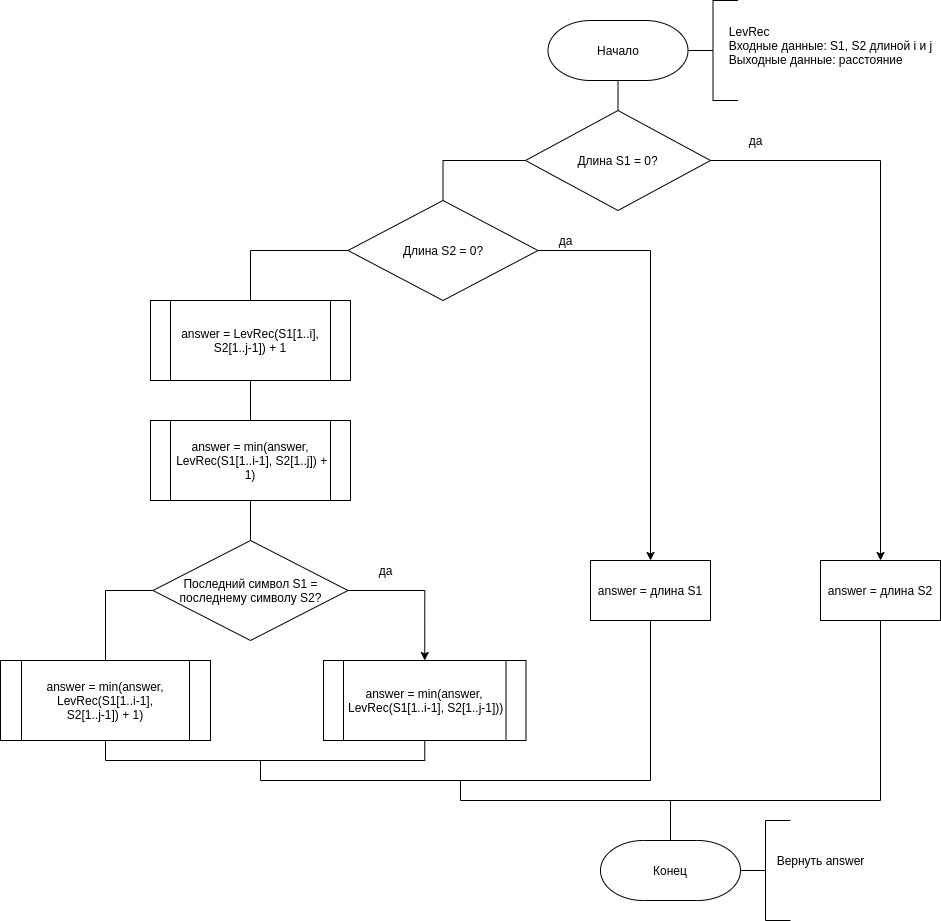
\includegraphics[scale=0.51]{schemes/LevRec.jpg}
	\caption{Схема рекурсивного алгоритма нахождения расстояния Левенштейна}
	\label{scheme:levrec}
\end{figure}

\begin{figure}[h]
	\centering
	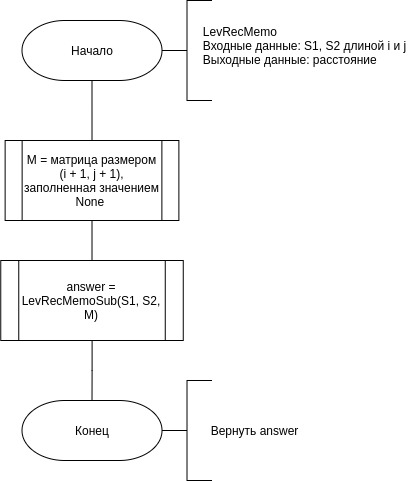
\includegraphics[scale=0.8]{schemes/LevRecMemo.jpg}
	\caption{Схема рекурсивного алгоритма нахождения расстояния Левенштейна с кэшированием}
	\label{scheme:levrecmemoutter}
\end{figure}
+

\begin{figure}[h]
	\centering
	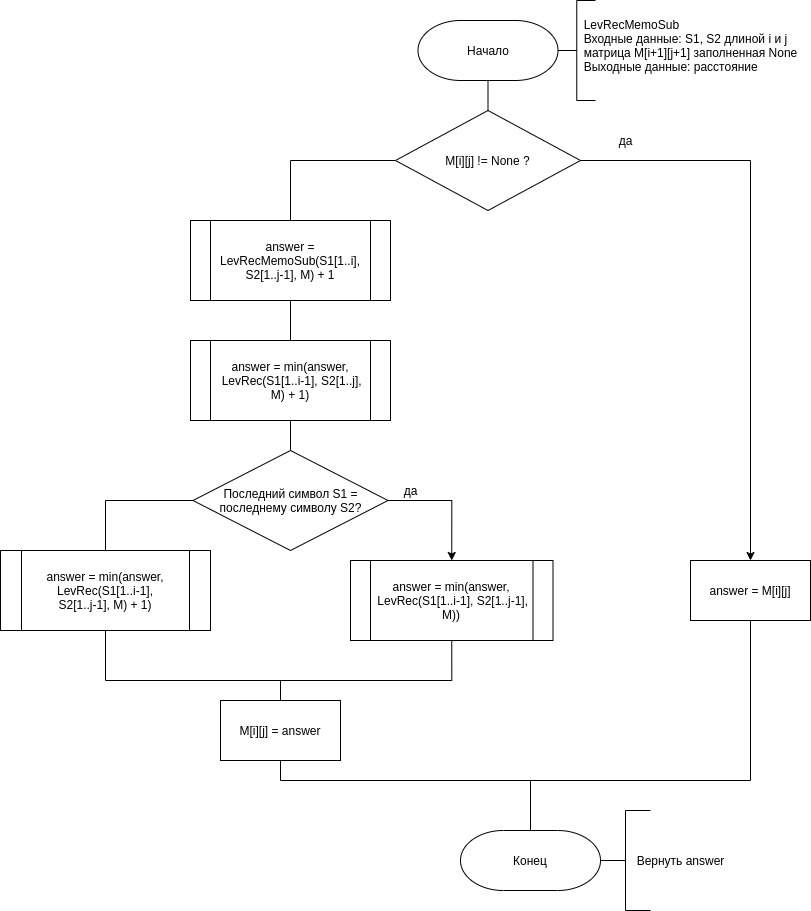
\includegraphics[scale=0.56]{schemes/LevRecMemoSub.jpg}
	\caption{Схема процедуры рекурсивного алгоритма нахождения расстояния Левенштейна с кэшированием}
	\label{scheme:levrecmeminner}
\end{figure}


\begin{figure}[h]
	\centering
	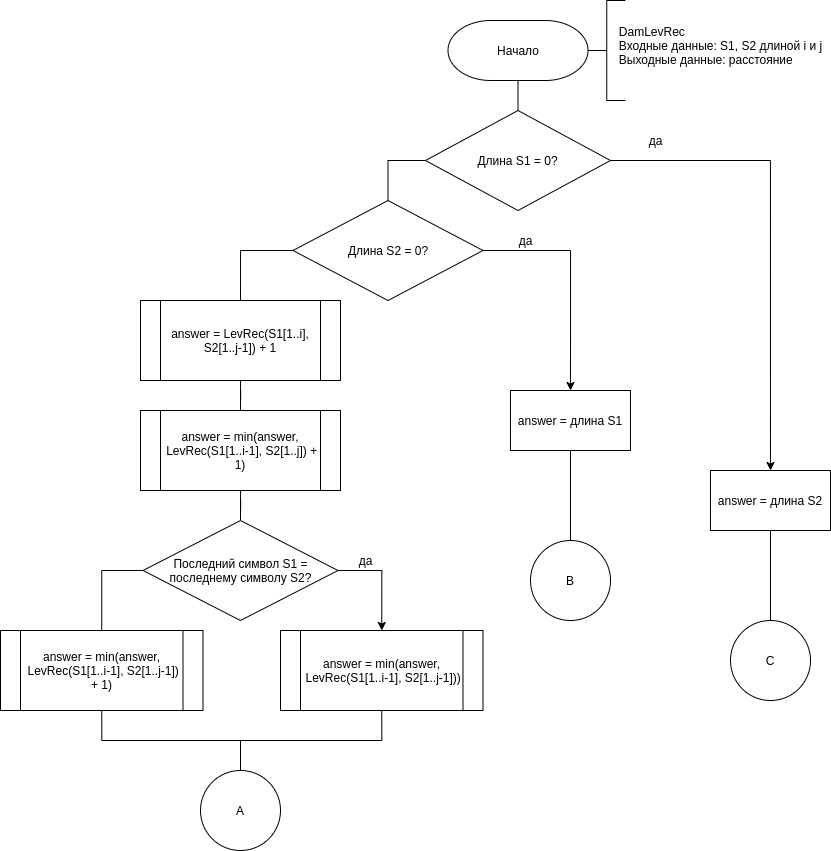
\includegraphics[scale=0.58]{schemes/DamLevRecTop.jpg}
	\caption{Схема рекурсивного алгоритма нахождения расстояния Дамерау-Левенштейна}
	\label{scheme:damlevrectop}
\end{figure}

\begin{figure}[h]
	\centering
	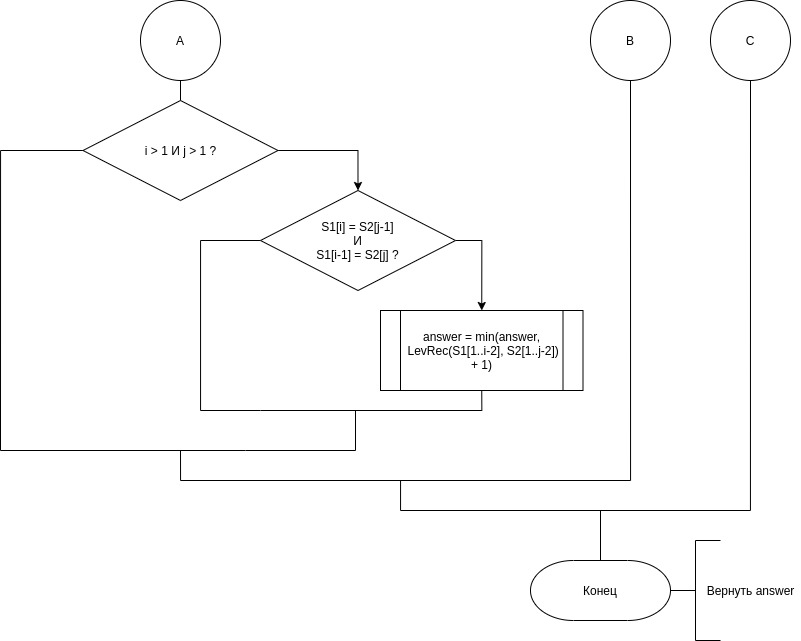
\includegraphics[scale=0.6]{schemes/DamLevRecBottom.jpg}
	\caption{Продолжение схемы рекурсивного алгоритма нахождения расстояния Дамерау-Левенштейна}
	\label{scheme:damlevrecbottom}
\end{figure}

\begin{figure}[h]
	\centering
	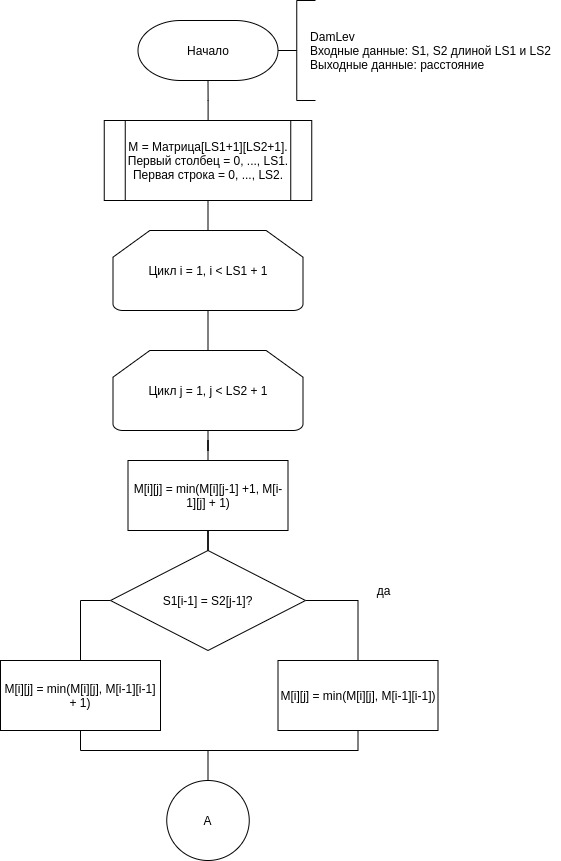
\includegraphics[scale=0.7]{schemes/DamLevTop.jpg}
	\caption{Схема матричного алгоритма нахождения расстояния Дамерау-Левенштейна}
	\label{scheme:damlevmatrtop}
\end{figure}

\begin{figure}[h]
	\centering
	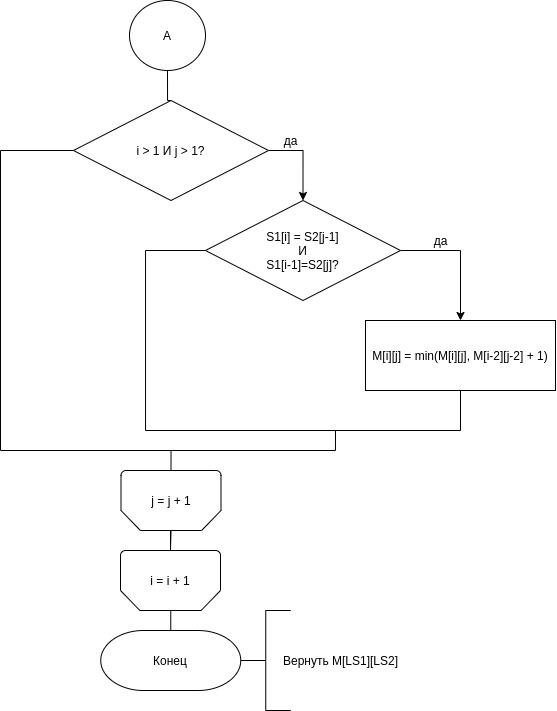
\includegraphics[scale=0.7]{schemes/DamLevBottom.jpg}
	\caption{Продолжение схемы матричного алгоритма нахождения расстояния Дамерау-Левенштейна}
	\label{scheme:damlevmatrbottom}
\end{figure}

\section{Вывод}
	На основе теоретических данных, полученные в аналитическом разделе были построены схемы иследуеммых  алгоритмов.
